\section{How much information is in the magnitude and the location of filter responses?}
\label{sec-where-info}
For studying the importance of location and the magnitude of filter responses, we constructed a set of ablations (described in fig \ref{fig:features}) and the studied their effect under the experimental conditions of image classification (see table \ref{table:class-ablation}) and object detection (see table\ref{table:det-ablation}).

\begin{figure}[t!]
\centering
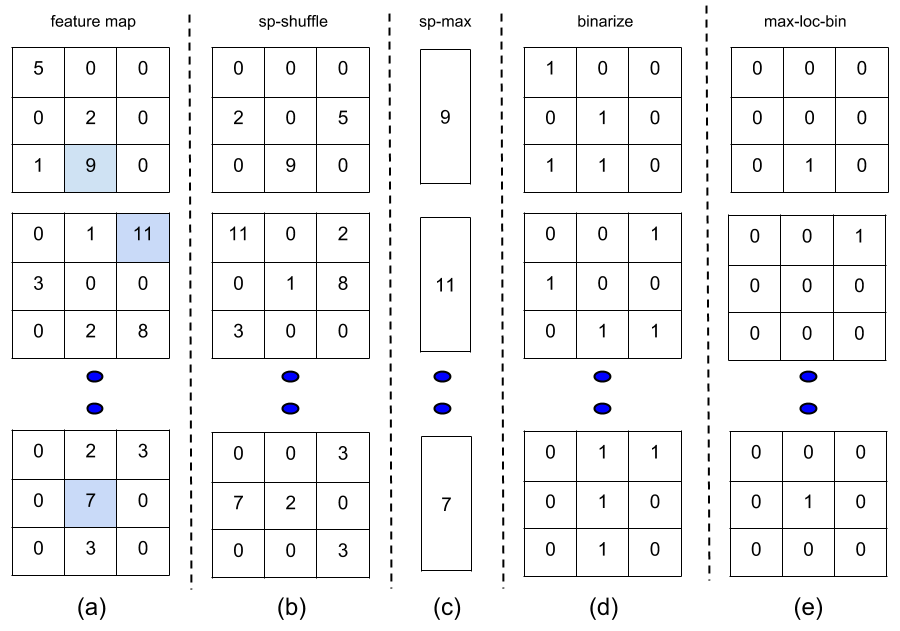
\includegraphics[height=6.5cm]{images/features1.png}
\caption{(a) For illustration, consider the output of a hypothetical layer of size k*k*N (k=3 for convolutional layers and k=1 for FC layers), which has N filters and their responses at k*k spatial locations. Linear SVMs were trained (one for each layer) after vectorizing (i.e. x(:) in matlab) features into a one-dimensional vector of length k*k*N to measure performance of different layers. Next, feature ablations as described below were applied before training SVMs and performance was compared against the un-ablated features. The set of k*k locations for each filter is called its feature map. (b) \textit{spatial-shuffle}(sp-shuffle) -  A random permutation is applied to the set of k*k activations associated with each feature map. Different images see different permutations. (c)\textit{spatial max}(sp-max): For each feature map, the maximum value is selected from the set of k*k activations. (d)\textit{binarization}(bin) Feature dimensions with value $>0$ are set to 1 and others to 0.}
\label{fig:features}
\end{figure}

\subsection{How important is the magnitude of activation ?}
\label{sub:imp-mag}
\setlength{\tabcolsep}{2pt}
\begin{table}[t!]
\begin{center}
\caption{Percentage non-zeros (sparsity) in features of various layers of CNN.}
\label{table:sparse}
\scalebox{1}{
\begin{tabular}{|c|c|c|c|c|c|c|}
\hline
conv-1 & conv-2 & conv-3 & conv-4 & conv-5 & fc-6 & fc-7 \\
\hline
$87.5 \pm 4.4$ & $44.5 \pm 4.4$ & $31.8 \pm 2.4$ & $32.0 \pm 2.7$ & $27.7 \pm 5.0$ & $16.1 \pm 3.0$ & $21.6 \pm 4.9$ \\
\hline
\end{tabular}}
\end{center}
\end{table}
\setlength{\tabcolsep}{1.4pt}

Binarization leads to loss of information contained in the magnitude of filter responses. We report that this leads to negligible decline in performance for both classification and detection (tables \ref{table:class-ablation}, \ref{table:det-ablation}). Further, the sparsity of CaffeNet features are reported in table \ref{table:sparse}. Notice, that the fc layers are quite sparse. A lot of work in image retrieval (NEED REF) focuses on finding sparse binary features - and our results indicate that one can get these `for free' from CNN features. 

\subsection{How important is where a filter activates?}
\label{sub:imp-loc}
The \textit{sp-max} and \textit{sp-shuffle} are two ablations which devoid the feature vector of the location of the filter response. For image classification, these lead to a large difference in performance between original and ablated conv-1 features, but gradually decreasing difference for higher layers (table \ref{table:class-ablation}). Infact, the performance of conv-5 after \textit{sp-max} is close to the original performance. This indicates, that a lot of information important for classification is encoded in the activation of the filters and not necessarily in the pattern of their activations. However, for detection \textit{sp-max} (tables \ref{table:det-ablation}) leads to a large drop in performance. 
This may not be surprising as in contrast to classification, for detection we need precise localization.

\setlength{\tabcolsep}{4pt}
\begin{table}[t!]
\begin{center}
\caption{Ablation study on PASCAL Image Classification (see fig \ref{fig:features})}
\label{table:class-ablation}
\begin{tabular}{lccccc}
\hline\noalign{\smallskip}
layer & no-ablation & bin & sp-shuffle & sp-max & sp-max-bin \\
\noalign{\smallskip}
\hline
\noalign{\smallskip}
conv-1 & $25.1 \pm 0.5$ & $17.7 \pm 0.2$ & $15.1 \pm 0.3$ & $25.4 \pm 0.5$ & $8.3  \pm 0.2$  \\ 
conv-2 & $45.3 \pm 0.5$ & $43.0 \pm 0.6$ & $32.9 \pm 0.7$ & $40.1 \pm 0.3$ & $11.7 \pm 0.3$  \\ 
conv-3 & $50.7 \pm 0.6$ & $47.2 \pm 0.6$ & $41.0 \pm 0.8$ & $54.1 \pm 0.5$ & $12.3 \pm 0.3$ \\
conv-4 & $54.5 \pm 0.7$ & $51.5 \pm 0.7$ & $45.2 \pm 0.8$ & $57.0 \pm 0.5$ & $11.3 \pm 0.2$  \\
conv-5 & $65.6 \pm 0.6$ & $60.8 \pm 0.7$ & $59.5 \pm 0.4$ & $62.5 \pm 0.6$ & $28.0 \pm 0.3$ \\
fc-6   & $71.7 \pm 0.3$ & $71.5 \pm 0.4$ &  -             &  -        &  -    \\
fc-7   & $74.1 \pm 0.3$ & $73.7 \pm 0.4$ &  -             &  -        &  -   \\
\hline
\end{tabular}
\end{center}
\end{table}
\setlength{\tabcolsep}{1.4pt}

\setlength{\tabcolsep}{1pt}
\begin{table}[t!]
\begin{center}
\caption{Ablation study on PASCAL Object Detection using conv-5 features\cite{Rcnn}. Binarization leads to negligible drop in performance whereas as \textit{sp-max} causes a large drop in performance.}
\label{table:det-ablation}
\scalebox{0.70}{
\begin{tabular}{l|cccccccccccccccccccc||c}
\hline\noalign{\smallskip}
Feature & aero & bike & bird & boat & bottle & bus & car & cat & chair & cow & table & dog & horse & mbike & person & plant & sheep & sofa & train & tv & mAP \\
\noalign{\smallskip}
\hline
conv-5  & 57.8 & 63.9 & 38.8 & 28.0 & 29.0 & 54.8 & 66.9 & 51.3 & 30.5 & 52.1 & 45.2 & 43.2 & 57.3 & 58.8 & 46.0 & 27.2 & 51.2 & 39.3 & 53.3 & 56.6 & 47.6 \\
bin & 57.9 & 61.3 & 32.6 & 24.7 & 27.5 & 55.0 & 64.7 & 49.8 & 25.3 & 47.4 & 44.5 & 40.3 & 54.6 & 56.4 & 43.6 & 27.1 & 48.4 & 41.6 & 54.3 & 57.6 & 45.7 \\
sp-max & 35.0 & 38.7 & 17.3 & 16.9 & 13.9 & 38.4 & 45.6 & 29.2 & 11.0 & 20.2 & 21.0 & 23.5 & 27.2 & 37.0 & 20.5 & 7.0 & 30.3 & 13.4 & 28.3 & 32.9 & 25.4 \\
\noalign{\smallskip}
\hline
\end{tabular}}
\end{center}
\end{table}
\setlength{\tabcolsep}{1.4pt}


\subsection{Discussion}
For classification although sp-max and binarization by themselves are not detrimental - their combination (sp-max-bin) is catastrophic to performance.